\section{Render\-Performer  Class Reference}
\label{classRenderPerformer}\index{RenderPerformer@{Render\-Performer}}
Perform 3D rendering using the SGI IRIS Performer library. 


{\tt \#include $<$renderpf.h$>$}

Inheritance diagram for Render\-Performer::\begin{figure}[H]
\begin{center}
\leavevmode
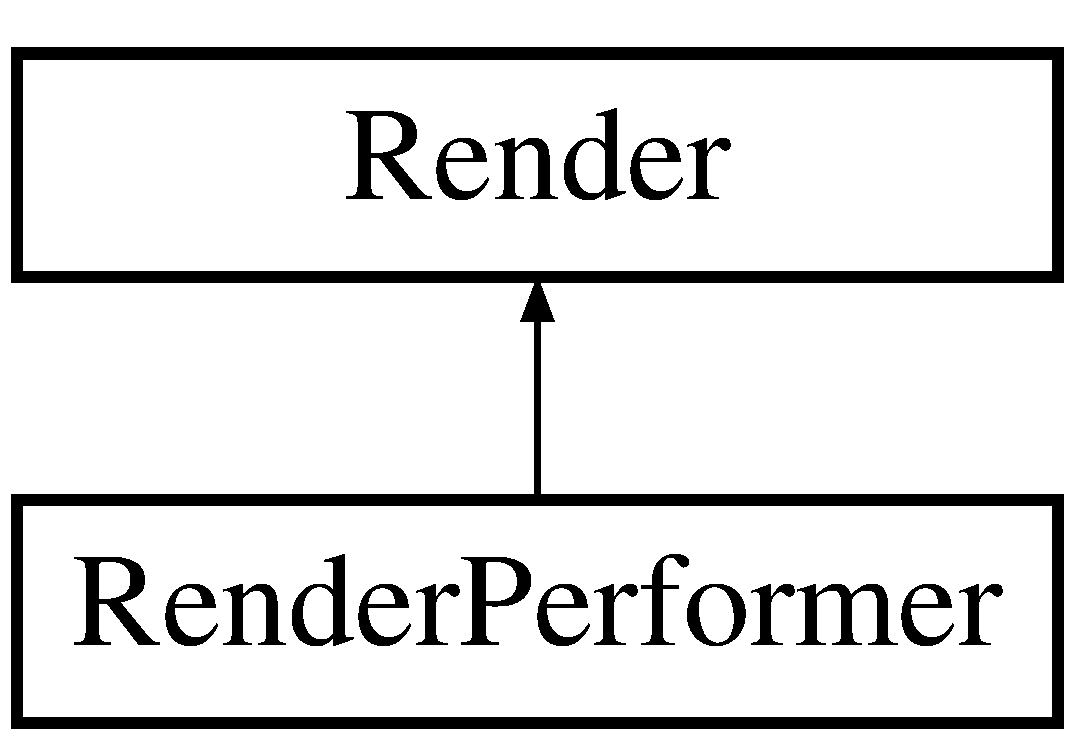
\includegraphics[height=2cm]{classRenderPerformer}
\end{center}
\end{figure}
\subsection*{Public Methods}
\begin{CompactItemize}
\item 
{\bf Render\-Performer} ()
\item 
{\bf Render\-Performer} (string filepath)
\item 
{\bf Render\-Performer} ({\bf Scene} $\ast$s, string filepath)
\item 
virtual {\bf $\sim$Render\-Performer} ()
\item 
virtual void {\bf Init} ()
\begin{CompactList}\small\item\em Initialized the renderer.\item\end{CompactList}\item 
virtual void {\bf Handle\-Events} ()
\begin{CompactList}\small\item\em Process IO events.\item\end{CompactList}\item 
virtual void {\bf Terminate} ()
\begin{CompactList}\small\item\em Implement functions upon termination of the renderer.\item\end{CompactList}\end{CompactItemize}
\subsection*{Protected Methods}
\begin{CompactItemize}
\item 
virtual void {\bf Show\-Current\-Animation\-Frame} ()
\begin{CompactList}\small\item\em Display the current animation frame in a rendering window.\item\end{CompactList}\item 
void {\bf Load\-Environment} (pf\-Group $\ast$env)
\item 
void {\bf Load\-Bodies} (pf\-Group $\ast$bodies)
\item 
pf\-Node$\ast$ {\bf Load\-Native\-Model} (string file, int colorindex)
\begin{CompactList}\small\item\em Load a model that is a {\bf list} {\rm (p.\,\pageref{classlist})} of 2D polygons or 3D triangles.\item\end{CompactList}\item 
void {\bf Make\-Bounding\-Box} (pf\-Geode $\ast$bound)
\item 
void {\bf Make\-Control\-Panel} (pf\-Group $\ast$con, pf\-DCS $\ast$pad)
\item 
void {\bf Get\-Current\-Mouse\-Pos} (double \&x, double \&y)
\item 
void {\bf Handle\-Key\-Input} ()
\item 
void {\bf Handle\-Mouse\-Events} ()
\item 
void {\bf Get\-Control\-Pad\-Size} (double \&padwidth\_\-l, double \&padwidth\_\-r, double \&padheight\_\-b, double \&padheight\_\-top)
\item 
void {\bf Norm\-Cross\-Product} (double v1[3], double v2[3], double out[3])
\end{CompactItemize}
\subsection*{Static Protected Methods}
\begin{CompactItemize}
\item 
void {\bf Draw\-Channel} (pf\-Channel $\ast$chan, void $\ast$data)
\end{CompactItemize}
\subsection*{Static Protected Attributes}
\begin{CompactItemize}
\item 
Shared\-Data$\ast$ {\bf Shared}
\end{CompactItemize}


\subsection{Detailed Description}
Perform 3D rendering using the SGI IRIS Performer library.



\subsection{Constructor \& Destructor Documentation}
\index{RenderPerformer@{Render\-Performer}!RenderPerformer@{RenderPerformer}}
\index{RenderPerformer@{RenderPerformer}!RenderPerformer@{Render\-Performer}}
\subsubsection{\setlength{\rightskip}{0pt plus 5cm}Render\-Performer::Render\-Performer ()}\label{classRenderPerformer_a0}


\index{RenderPerformer@{Render\-Performer}!RenderPerformer@{RenderPerformer}}
\index{RenderPerformer@{RenderPerformer}!RenderPerformer@{Render\-Performer}}
\subsubsection{\setlength{\rightskip}{0pt plus 5cm}Render\-Performer::Render\-Performer (string {\em filepath} = \char`\"{}\char`\"{})}\label{classRenderPerformer_a1}


\index{RenderPerformer@{Render\-Performer}!RenderPerformer@{RenderPerformer}}
\index{RenderPerformer@{RenderPerformer}!RenderPerformer@{Render\-Performer}}
\subsubsection{\setlength{\rightskip}{0pt plus 5cm}Render\-Performer::Render\-Performer ({\bf Scene} $\ast$ {\em s}, string {\em filepath})}\label{classRenderPerformer_a2}


\index{RenderPerformer@{Render\-Performer}!~RenderPerformer@{$\sim$RenderPerformer}}
\index{~RenderPerformer@{$\sim$RenderPerformer}!RenderPerformer@{Render\-Performer}}
\subsubsection{\setlength{\rightskip}{0pt plus 5cm}Render\-Performer::$\sim$Render\-Performer ()\hspace{0.3cm}{\tt  [inline, virtual]}}\label{classRenderPerformer_a3}




\subsection{Member Function Documentation}
\index{RenderPerformer@{Render\-Performer}!DrawChannel@{DrawChannel}}
\index{DrawChannel@{DrawChannel}!RenderPerformer@{Render\-Performer}}
\subsubsection{\setlength{\rightskip}{0pt plus 5cm}void Render\-Performer::Draw\-Channel (pf\-Channel $\ast$ {\em chan}, void $\ast$ {\em data})\hspace{0.3cm}{\tt  [static, protected]}}\label{classRenderPerformer_e0}


\index{RenderPerformer@{Render\-Performer}!GetControlPadSize@{GetControlPadSize}}
\index{GetControlPadSize@{GetControlPadSize}!RenderPerformer@{Render\-Performer}}
\subsubsection{\setlength{\rightskip}{0pt plus 5cm}void Render\-Performer::Get\-Control\-Pad\-Size (double \& {\em padwidth\_\-l}, double \& {\em padwidth\_\-r}, double \& {\em padheight\_\-b}, double \& {\em padheight\_\-top})\hspace{0.3cm}{\tt  [protected]}}\label{classRenderPerformer_b9}


\index{RenderPerformer@{Render\-Performer}!GetCurrentMousePos@{GetCurrentMousePos}}
\index{GetCurrentMousePos@{GetCurrentMousePos}!RenderPerformer@{Render\-Performer}}
\subsubsection{\setlength{\rightskip}{0pt plus 5cm}void Render\-Performer::Get\-Current\-Mouse\-Pos (double \& {\em x}, double \& {\em y})\hspace{0.3cm}{\tt  [protected]}}\label{classRenderPerformer_b6}


\index{RenderPerformer@{Render\-Performer}!HandleEvents@{HandleEvents}}
\index{HandleEvents@{HandleEvents}!RenderPerformer@{Render\-Performer}}
\subsubsection{\setlength{\rightskip}{0pt plus 5cm}void Render\-Performer::Handle\-Events ()\hspace{0.3cm}{\tt  [virtual]}}\label{classRenderPerformer_a5}


Process IO events.



Reimplemented from {\bf Render} {\rm (p.\,\pageref{classRender_a5})}.\index{RenderPerformer@{Render\-Performer}!HandleKeyInput@{HandleKeyInput}}
\index{HandleKeyInput@{HandleKeyInput}!RenderPerformer@{Render\-Performer}}
\subsubsection{\setlength{\rightskip}{0pt plus 5cm}void Render\-Performer::Handle\-Key\-Input ()\hspace{0.3cm}{\tt  [protected]}}\label{classRenderPerformer_b7}


\index{RenderPerformer@{Render\-Performer}!HandleMouseEvents@{HandleMouseEvents}}
\index{HandleMouseEvents@{HandleMouseEvents}!RenderPerformer@{Render\-Performer}}
\subsubsection{\setlength{\rightskip}{0pt plus 5cm}void Render\-Performer::Handle\-Mouse\-Events ()\hspace{0.3cm}{\tt  [protected]}}\label{classRenderPerformer_b8}


\index{RenderPerformer@{Render\-Performer}!Init@{Init}}
\index{Init@{Init}!RenderPerformer@{Render\-Performer}}
\subsubsection{\setlength{\rightskip}{0pt plus 5cm}void Render\-Performer::Init ()\hspace{0.3cm}{\tt  [virtual]}}\label{classRenderPerformer_a4}


Initialized the renderer.



Reimplemented from {\bf Render} {\rm (p.\,\pageref{classRender_a4})}.\index{RenderPerformer@{Render\-Performer}!LoadBodies@{LoadBodies}}
\index{LoadBodies@{LoadBodies}!RenderPerformer@{Render\-Performer}}
\subsubsection{\setlength{\rightskip}{0pt plus 5cm}void Render\-Performer::Load\-Bodies (pf\-Group $\ast$ {\em bodies})\hspace{0.3cm}{\tt  [protected]}}\label{classRenderPerformer_b2}


\index{RenderPerformer@{Render\-Performer}!LoadEnvironment@{LoadEnvironment}}
\index{LoadEnvironment@{LoadEnvironment}!RenderPerformer@{Render\-Performer}}
\subsubsection{\setlength{\rightskip}{0pt plus 5cm}void Render\-Performer::Load\-Environment (pf\-Group $\ast$ {\em env})\hspace{0.3cm}{\tt  [protected]}}\label{classRenderPerformer_b1}


\index{RenderPerformer@{Render\-Performer}!LoadNativeModel@{LoadNativeModel}}
\index{LoadNativeModel@{LoadNativeModel}!RenderPerformer@{Render\-Performer}}
\subsubsection{\setlength{\rightskip}{0pt plus 5cm}pf\-Node $\ast$ Render\-Performer::Load\-Native\-Model (string {\em file}, int {\em colorindex})\hspace{0.3cm}{\tt  [protected]}}\label{classRenderPerformer_b3}


Load a model that is a {\bf list} {\rm (p.\,\pageref{classlist})} of 2D polygons or 3D triangles.

\index{RenderPerformer@{Render\-Performer}!MakeBoundingBox@{MakeBoundingBox}}
\index{MakeBoundingBox@{MakeBoundingBox}!RenderPerformer@{Render\-Performer}}
\subsubsection{\setlength{\rightskip}{0pt plus 5cm}void Render\-Performer::Make\-Bounding\-Box (pf\-Geode $\ast$ {\em bound})\hspace{0.3cm}{\tt  [protected]}}\label{classRenderPerformer_b4}


\index{RenderPerformer@{Render\-Performer}!MakeControlPanel@{MakeControlPanel}}
\index{MakeControlPanel@{MakeControlPanel}!RenderPerformer@{Render\-Performer}}
\subsubsection{\setlength{\rightskip}{0pt plus 5cm}void Render\-Performer::Make\-Control\-Panel (pf\-Group $\ast$ {\em con}, pf\-DCS $\ast$ {\em pad})\hspace{0.3cm}{\tt  [protected]}}\label{classRenderPerformer_b5}


\index{RenderPerformer@{Render\-Performer}!NormCrossProduct@{NormCrossProduct}}
\index{NormCrossProduct@{NormCrossProduct}!RenderPerformer@{Render\-Performer}}
\subsubsection{\setlength{\rightskip}{0pt plus 5cm}void Render\-Performer::Norm\-Cross\-Product (double {\em v1}[3], double {\em v2}[3], double {\em out}[3])\hspace{0.3cm}{\tt  [protected]}}\label{classRenderPerformer_b10}


\index{RenderPerformer@{Render\-Performer}!ShowCurrentAnimationFrame@{ShowCurrentAnimationFrame}}
\index{ShowCurrentAnimationFrame@{ShowCurrentAnimationFrame}!RenderPerformer@{Render\-Performer}}
\subsubsection{\setlength{\rightskip}{0pt plus 5cm}void Render\-Performer::Show\-Current\-Animation\-Frame ()\hspace{0.3cm}{\tt  [protected, virtual]}}\label{classRenderPerformer_b0}


Display the current animation frame in a rendering window.



Reimplemented from {\bf Render} {\rm (p.\,\pageref{classRender_b1})}.\index{RenderPerformer@{Render\-Performer}!Terminate@{Terminate}}
\index{Terminate@{Terminate}!RenderPerformer@{Render\-Performer}}
\subsubsection{\setlength{\rightskip}{0pt plus 5cm}void Render\-Performer::Terminate ()\hspace{0.3cm}{\tt  [virtual]}}\label{classRenderPerformer_a6}


Implement functions upon termination of the renderer.



Reimplemented from {\bf Render} {\rm (p.\,\pageref{classRender_a8})}.

\subsection{Member Data Documentation}
\index{RenderPerformer@{Render\-Performer}!Shared@{Shared}}
\index{Shared@{Shared}!RenderPerformer@{Render\-Performer}}
\subsubsection{\setlength{\rightskip}{0pt plus 5cm}Shared\-Data $\ast$ Render\-Performer::Shared\hspace{0.3cm}{\tt  [static, protected]}}\label{classRenderPerformer_q0}




The documentation for this class was generated from the following files:\begin{CompactItemize}
\item 
{\bf renderpf.h}\item 
{\bf renderpf.C}\end{CompactItemize}
